\documentclass[
	ddcfooter,
	german,
%	nototalpages,
%	handout
]{tudbeamer}

\usepackage[utf8]{inputenc}

\usepackage[babel, german=guillemets]{csquotes}
\usepackage{xspace}

\usepackage{listings}

\usepackage[style=numeric-verb, backend=bibtex]{biblatex}
\DeclareFieldFormat{urldate}{\space\tiny[#1]}
\addbibresource{../../references}
\addbibresource{additional}

\setbeamerfont{caption}{size=\tiny}

\graphicspath{ {./graphics/} }

\einrichtung{Fakultät Informatik}
\institut{Institut für Software- und Multimediatechnik}
\professur{Computergraphik und Visualisierung}

\title{Zwischenpräsentation}
\subtitle{KP Graphische Datenverarbeitung WS 14/15}
\author{Felix Mai}
\date{26. Januar 2015}

\newcommand{\blankline}{\newline\space\newline}
\newcommand{\arrow}{\ensuremath{\rightarrow}~}
\newcommand{\thus}{\item[\arrow]}
\newcommand{\zb}{z.\,B.\xspace}

\newcommand{\code}[1]{\texttt{#1}}


\begin{document}

\maketitle


\section{Einleitung}

\subsection{Aufgabenstellung}

\begin{frame}{Einleitung}{Aufgabenstellung}
\end{frame}

\subsection{Motivation}

\begin{frame}{Einleitung}{Motivation}
\end{frame}

\subsection{Setup}

\begin{frame}{Einleitung}{Setup}
\end{frame}

\subsection{Teilprobleme}

\begin{frame}{Einleitung}{Teilprobleme}
\end{frame}



\section{Jaco-Arm}

\begin{frame}{Jaco-Arm}
\end{frame}



\section{Kinect}

\begin{frame}{Kinect}
\end{frame}



\section{Erkennung}

\begin{frame}[b]
	\begin{figure}
		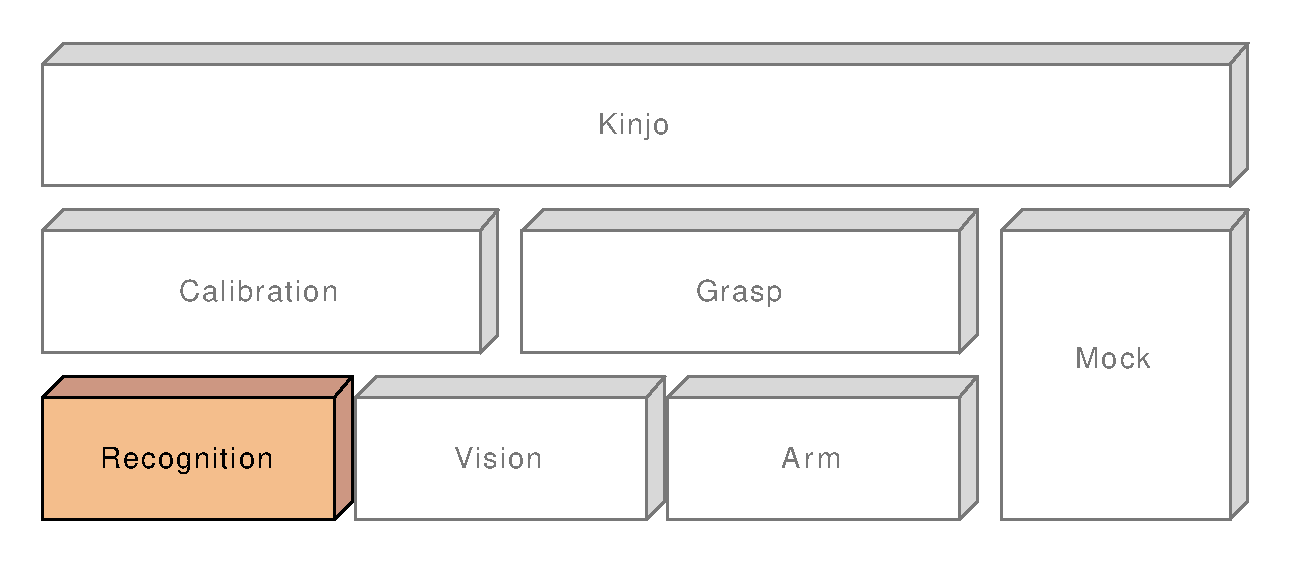
\includegraphics[width=0.8\textwidth]{nav_recognition}
	\end{figure}
	\vspace*{0.7cm}
\end{frame}

\begin{frame}[t]{Erkennung}
	\begin{itemize}
		\item Eingabe: RGB-Bild
		\item Ausgabe: XY-Pixel-Position und Radius des erkannten
			Kalibrierungsobjektes
		\item Aktuell nur für Kreisförmige Objekte beliebig einstellbarer
			Farbe
		\item Objekt bzw. Farbe muss eindeutig erkennbar sein
	\end{itemize}
\end{frame}

\begin{frame}[t]{Erkennung}
	\begin{block}{Abfolge}
		\begin{columns}[t]
			\begin{column}{0.4\textwidth}
				\only<1>{
					\begin{figure}
						
\includegraphics[width=\textwidth]{recognition_Depth}
					\end{figure}
				}
				\only<2-4>{
					\begin{enumerate}
						\item<2-4> Konvertierung von RGB- nach HSV-Farbraum (für einfacheres Maskieren des
							Farbbereiches in Schritt 2)
						\item<3-4> Maskieren der Pixel im erwarteten Farbbereich
						\item<4> Morphologische Operationen zum Entfernen von zu kleinen oder
							nicht kreisförmigen Strukturen
					\end{enumerate}
				}
				\only<5->{
					\begin{enumerate}
						\setcounter{enumi}{3}
						\item<5-> Blur für bessere Kreiserkennung
						\item<6-> Kreiserkennung mittels Hough-Transformation.
						\item<7-> Rating aller erkannten Objekte und Rückgabe des besten.
					\end{enumerate}
				}
			\end{column}
			\begin{column}{0.4\textwidth}
				\begin{figure}
					\includegraphics<1>[width=\textwidth]{recognition_RGB}
					\includegraphics<2>[width=\textwidth]{recognition_HSV}
					\includegraphics<3>[width=\textwidth]{recognition_Mask}
					\includegraphics<4>[width=\textwidth]{recognition_MaskFilter}
					\includegraphics<5>[width=\textwidth]{recognition_MaskFilterBlur}
					\includegraphics<6->[width=\textwidth]{recognition_RecognitionResult}
				\end{figure}
			\end{column}
		\end{columns}
	\end{block}
\end{frame}



\section{Kalibrierung}

\begin{frame}[b]
	\begin{figure}
		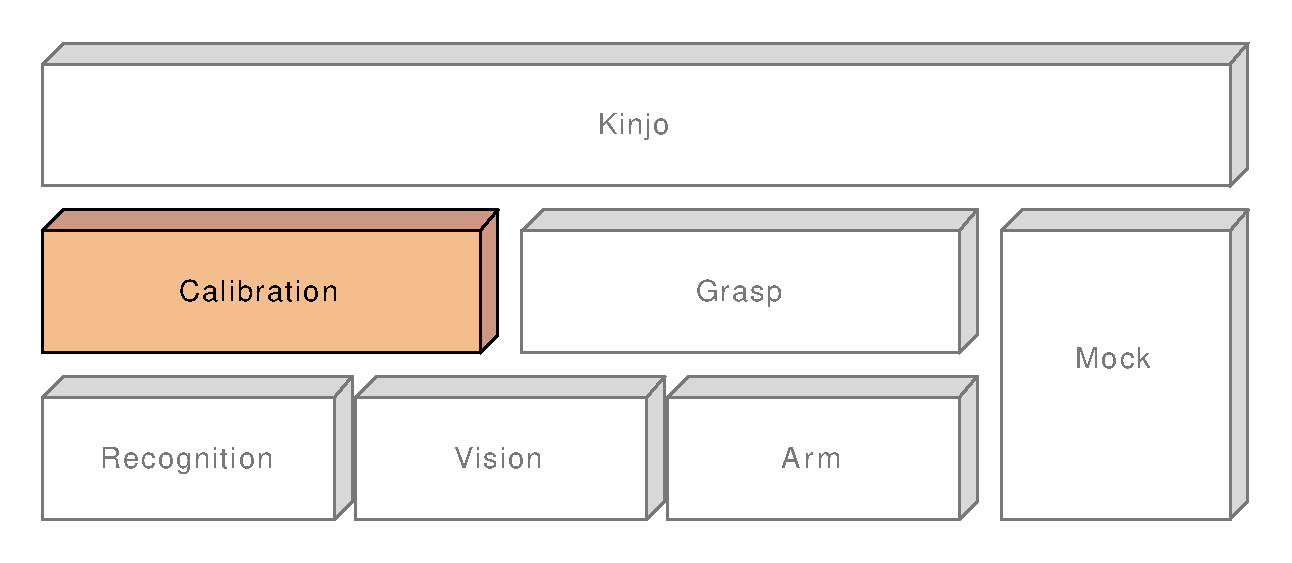
\includegraphics[width=0.8\textwidth]{nav_calibration}
	\end{figure}
	\vspace*{0.7cm}
\end{frame}

\begin{frame}[t]{Kinect}
	\begin{block}{Kalibrierung}
		\begin{itemize}
			\item Asynchron zur Hauptanwendung, damit Bildausgabe weiter läuft
			\item Fährt $P$ (zufällige) Punkte an
			\item Lässt an diesen Punkten die Hand in $R$ unterschiedliche
				Rotationen fahren
			\item Nimmt $K$ Bilder auf und versucht jeweils das
				Kalibrierungsobjekt zu erkennen
			\item Filtert aus den $R \cdot K$ Ergebnispunkten Ausreißer heraus
				und mittelt das Ergebnis
			\item Speichert die (maximal) $P$ Korrespondenzen von Arm-Position
				und erkannter Kinect-Position
			\item Berechnung der Starrkörpertransformation mittels
				\enquote{Least-Squares Rigid Motion Using SVD}
				\cite{sorkine2009lsrmusvd}
		\end{itemize}
	\end{block}
\end{frame}



\section{Greifen}

\begin{frame}[b]
	\begin{figure}
		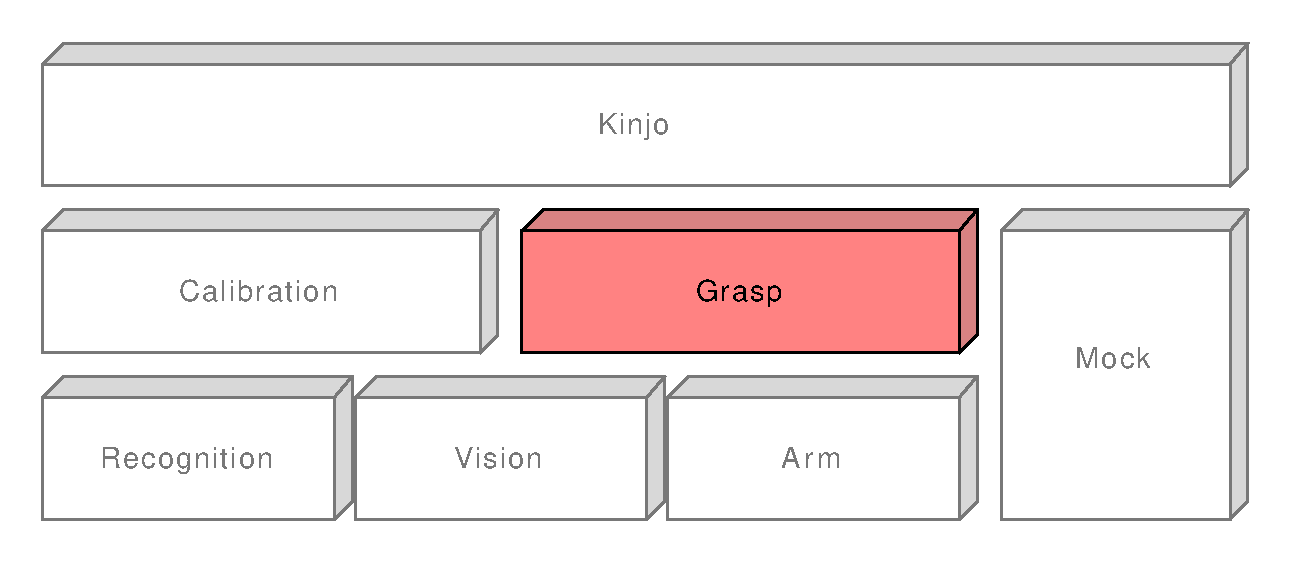
\includegraphics[width=0.8\textwidth]{nav_grasp}
	\end{figure}
	\vspace*{0.7cm}
\end{frame}

\begin{frame}[t]{Greifen}
	\vspace*{2cm}
	\centerline{\large\emph{Noch ausstehend}}
\end{frame}



\section{Ausblick}

\begin{frame}{Ausblick}
\end{frame}



\section{Demonstation}

\begin{frame}[t]
	\vspace*{2.5cm}
	\centerline{\huge{Demonstration des}}
	\centerline{\huge{aktuellen Standes}}
\end{frame}

\begin{frame}[t]
	% states diagram, colors
	% - finished: #22AD36
	% - current:  #E87B14
	% - disabled: #AAAAAA
	\begin{figure}
		\includegraphics<1>[width=0.7\textwidth]{states}
		\includegraphics<2>[width=0.7\textwidth]{states_1}
		\includegraphics<3>[width=0.7\textwidth]{states_2}
		\includegraphics<4>[width=0.7\textwidth]{states_3}
		\caption{Zustände der Kinjo-Anwendung}
	\end{figure}
\end{frame}




\begin{frame}[t]
	\vspace*{2.5cm}
	\centerline{\huge{Fragen oder Anmerkungen?}}
\end{frame}


\section*{References}

\begin{frame}[t]
	\frametitle*{References}
	\renewcommand*{\bibfont}{\tiny}
	\nocite{*}
	\printbibliography[title=References]
\end{frame}

\end{document}

